\documentclass[a4paper,12pt]{article}
\usepackage[a4paper,top=1.3cm,bottom=2cm,left=1.5cm,right=1.5cm,marginparwidth=0.75cm]{geometry}
\usepackage{cmap}
\usepackage{mathtext}
\usepackage[T2A]{fontenc}
\usepackage[utf8]{inputenc}
\usepackage[english,russian]{babel}
\usepackage{siunitx}

\usepackage{graphicx}

\usepackage{wrapfig}
\usepackage{tabularx}
\usepackage{multirow}

\usepackage{hyperref}
\usepackage[rgb]{xcolor}
\hypersetup{
colorlinks=true,urlcolor=blue
}
\usepackage{amsmath,amsfonts,amssymb,amsthm,mathtools}
\usepackage{icomma}
\mathtoolsset{showonlyrefs=false}
\usepackage{euscript}
\usepackage{mathrsfs}
\DeclareMathOperator{\sgn}{\mathop{sgn}}
\newcommand*{\hm}[1]{#1\nobreak\discretionary{}
{\hbox{$\mathsurround=0pt #1$}}{}}

%%% Заголовок
\author{Макаров Лев Евгеньевич}
\title{Лабораторная работа №2.2.1

Исследование взаимной диффузии газов
}
\date{\today}

\begin{document}

\begin{titlepage}
	\begin{center}
		{\large МОСКОВСКИЙ ФИЗИКО-ТЕХНИЧЕСКИЙ ИНСТИТУТ (НАЦИОНАЛЬНЫЙ ИССЛЕДОВАТЕЛЬСКИЙ УНИВЕРСИТЕТ)}
	\end{center}
	\begin{center}
		{\large Физтех-школа фотоники, электроники и молекулярной физики}
	\end{center}
	
	
	\vspace{4.5cm}
	{\huge
		\begin{center}
			{\bf Отчёт о выполнении лабораторной работы 2.2.1}\\
			Исследование взаимной диффузии газов
		\end{center}
	}
	\vspace{2cm}
	\begin{flushright}
		{\LARGE Автор:\\ Макаров Лев Евгеньевич \\
			\vspace{0.2cm}
			Б04-306}
	\end{flushright}
	\vspace{8cm}
	\begin{center}
		Долгопрудный 2024
	\end{center}
\end{titlepage}

\section{Введение}

\textbf{Цель работы:} 
\begin{enumerate}
	\item регистрация зависимости концентрации гелия в воздухе от времени с помощью датчиков теплопроводности при разных начальных давлениях смеси газов
    \item определение коэффициента диффузии по результатам измерений
\end{enumerate}

\textbf{В работе используются:} 
\begin{itemize}
    \item измерительная установка
    \item форвакуумный насос
    \item баллон с газом (гелий)
    \item манометр
    \item источник питания
    \item магазин сопротивлений
    \item гальванометр
    \item секундомер
\end{itemize}
\medskip

\section{Теоретические сведения}


Диффузия - самопроизвольное взаимное проникновение веществ друг в друга, происходящее вследствие хаотичного теплового движения молекул. При перемешивании молекул разного сорта говорят о взаимной (или концентрационной) диффузии.

В системе, состоящей из двух компонентов, плотность потока вещества в результате взаимной диффузии описывается законом Фика:

\begin{equation}
    j_a = -D_{ab}\frac{\partial n_a}{\partial x}, j_b = -D_{b_a} \frac{\partial n_b}{\partial x}
\end{equation}

где $D_{ab} = D_{ba} = D$ -- коэффициент взаимной диффузии компонентов, $j_{ab}$ = плотности потока частиц соответствующего сорта (количество частиц, пересекающих единичную площадку в единицу времени).\\

В работе исследуется диффузия примеси лёгкого газа (гелия) на фоне воздуха, поэтому концентрация воздуха в опыте значительно больше концентрации гелия, и её относительное изменение незначительно. В процессе работы будет описываться только диффузия примеси гелия на стационарном фоне воздуха.

Проведём теоретическую оценку величины коэффициента взаимной диффузии. В работа мала концентрация гелия, более того, масса атомов гелия много меньше массы молекул, составляющих воздух. При таких условиях перемешивание газов в эксперимента можно рассматривать как диффузию гелия на стационарном форне воздуха. Тогда коэффициент диффузии приблизительно равен

\begin{equation}\label{eq:2}
    D = \frac{1}{3}\lambda \bar v
\end{equation}

где $\lambda$ -- длина свободного пробега частиц гелия, $\bar v = \sqrt{\frac{8kT}{\pi m}}$ -- их средняя тепловая скорость. В общем случае необходимо считать $\lambda = \frac{1}{n_\Sigma \sigma}$, где $n_\Sigma = n_{He} + n_B = \frac{P_\Sigma}{kT}$ - полная концентрация частиц, $\sigma$ -- среднее сечение столкновения частиц гелия с воздухом. Также  $\bar v = \sqrt{\frac{8kT}{\pi \mu}}$ -- средняя относитель. Таким образом, теоретическая оценка предполагает, что коэффициент диффузии не зависит от пропорция элементов, а обратно пропорционален давлению $D \propto \frac{1}{P_\Sigma}$. \\

Рассмотрим процесс выравнивания концентрации в установке, она зависит от координат и времени во всей установке. Объём соединительной трубки мал по сравнению с с объёмами сосудов. Поэтому концентрации газов можно считать постоянной по всему объёму сосудов; считаем, что процесс выравнивания происходит только за счёт диффузии в трубке и является стационарным (так как считаем стационарным поток частиц). Величина этого стационарного потока $J = -DS\frac{\partial n}{\partial x}$, и он одинаковый во всём сечении трубки, тогда $n(x)$ - линейная функция координаты и $\frac{dn}{dx} = \frac{\triangle n}{l}$ (l -- длина трубки), получаем 

\begin{equation}
    J = -DS \frac{n_1-n_2}{l}
\end{equation}

Предположим, что установился линейный профиль концентрации и полученное соотношение справедливо в любой момент времени. Получаем квазистационарное приближение зависимости концентраций $n_1$ и $n_2$ от времени.

Через $\Delta n_1$ и $\Delta n_2$ обозначим изменения концентрации в объёмах $V_1$ и $V_1$ за время $\Delta t$. Тогда $V_1 \Delta n_1$ - изменение количества компонента в объёме $V_1$, а $V_2 \Delta n_2$ - изменение количества этого компонента в объёме $V_2$. По закону сохранения вещества следует, что $V_1 \Delta n_1 + V_2 \Delta n_2 = const$, поэтому $V_1 \Delta n_1 = - V_2 \Delta n_2$. Эти изменения происходят вследствие диффузии, поэтому

\begin{equation}
    V_1 \Delta n_1 = - V_2 \Delta n_2 = J \Delta t = -DS \frac{n_1-n_2}{l} \Delta t
\end{equation}

Делим равенство на $\Delta t$

\begin{equation}
    V_1 \frac{dn_1}{dt} = -DS\frac{n_1-n_2}{l}, V_2 \frac{dn_2}{dt} = -DS\frac{n_1-n_2}{l}
\end{equation}

Делим первое уравнение на $V_1$, второе на $V_2$, вычтем равенства друг из друга:

\begin{equation}
    \frac{dn_1}{dt}- \frac{dn_2}{dt} = - \frac{n_1-n_2}{l}DS(\frac{1}{V_1} +\frac{1}{V_2} )
\end{equation}

Введём новую переменную $\Delta n = n_1-n_2$, проинтегрируем уравнение, получим

\begin{equation}\label{eq:7}
    \Delta n = \Delta n_0 e^{(-t/\tau)}
\end{equation}

где $\Delta n_0$ - разность концентраций примеси в начльный момент времени, а

\begin{equation}\label{eq:8}
    \tau = \frac{V_1 V_2}{V_1 + V_2} \frac {l}{SD}
\end{equation}

Видим, что разность концентраций убывает по экспоненциальному закону и тем быстрее, чем меньше $\tau$ - величина, определяющаяся геометрическими параметрами установки и величиной коэффициента диффузии.

Для проверки применимости квазистационарного течения убедимся, что время $\tau$ много больше характерного времени диффузии одной частицы вдоль трубки длиной l: $\displaystyle t_{diff} \sim \frac{l^2}{D} \ll \tau$.

Для измерения концентраций применяются датчики теплопроводности $D_1$ и $D_2$ (см. рис. \ref{picture:ustan}) и используется зависимость теплопроводности газовой смеси от её состава. Тонкая проволока радиуса $r$, протянутая вдоль оси цилиндра радиуса $R$, нагревается током. Тепло от проволоки к стенке цилиндра передаётся главным образом вспледствие теплороводности газа, находящегося внутри цилиндра. Количество тепла переданного стенке цилиндра в единицу времени, определяется по формуле

\begin{equation}
    Q = \kappa \frac{2\pi L}{ln (R/r)}(T_1-T_2)
\end{equation}

где $\kappa$ - теплопроводность, $L$ - длина нити, $T_1, T_2$ - температуры проволочки и стенки. При $Q = const$ температура проволоки и её сопротивление определяются теплопроводностью газа и, следовательно, его составом. Для измерения разности концентраций газов используется мостовая схема, представленная на рис. \ref{picture:scheme} (см. пункт 4).

В процессе диффузии разность концентраций убывает по экспоненциальному закону. По тому же закону изменяются во времени показания гальванометра:

\begin{equation}
    U = U_0 e^{(-t/\tau)}
\end{equation}

Измеряя экспериментально зависимость $U(t)$, можно получить характерное время процесса $\tau$, откуда определить коэффициент диффузии D.

\section{Оборудование и экспериментальные погрешности}

\textbf{Секундомер:} $\sigma_\text{s} = 0,003$ с \\
\textbf{Гальванометр:} $\sigma_\text{v} = 0.0003$ мВ \\

\subsection*{Эксперементальная установка}

Общий вид конструкции установки приведён на рис. \ref{picture:ustan}. Установка состоит из двух сосудов $V_1$ и $V_2$, соединённых краном $K_3$, форвакуумного насоса Ф.Н. с выключателем Т, манометра М и системы напуска гелия, состоящей из кранов $K_6, K'_6, K_7$. Кран $K_5$ позволяет соединять форвакуумны насос либо с установкой, либо с атмосферой. Сосуды $V_1$ и $V_2$ соединены трубкой длины $l$ и сечения $S$. Сосуды заполнены смесь двух газов при одинаковом давлении, но с различной концентрацией компонентов. Вследствие взаимной диффузии концентрации каждого из компонентов с течением времени выравниваются Между форвакуумным насосом и краном $K_5$ вставлен предохранительный баллон, защищающий кран и установку при неправильной её эксплуатации от попадания форвакуумного масла из насоса. Сосуды $V_1$ и $V_2$ можно соединять как с системой напуска гелия, так и с форвакуумным насосом. Для этот служат краны $K_1, K_2, K_4, K_5$. Манометр М регистрирует давление газа, до которого заполняют тот или иной сосуды. Кран $K_4$ изолирует форвакуумный насос от установки. Для подачи воздуха в установку служит кран $K_5$. Дополнительный кран $K'_6$ служит для вакуумной изоляции установки от системы подачи гелия. Краны $K_4, K_5, K'_6$ обладают повышенной вакуумплотностью и хорошо изолируют установку от протечек.

\begin{figure}[!h]
    \centering
    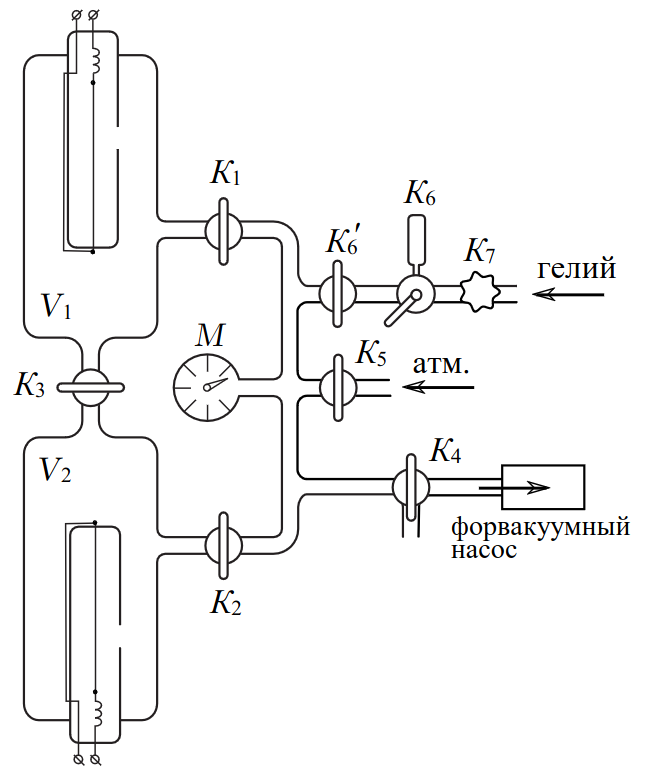
\includegraphics[width=9.5 cm]{ustan_C.png}
    \caption{Установка для исследования взаимной диффузии газов}
    \label{picture:ustan}
\end{figure}

Для измерения разности концентраций газов используется мостовая схема, представленная на рис. \ref{picture:scheme}. \\

Здесь $D_1, D_2$ - датчики теплопроводности, расположенные в сосудах $V_1$ и $V_2$. Сопротивления $R_1, R_2, R$ служат для установки прибора на нуль (балансировка моста). В одну из диагоналей моста включен гальванометр, к другой подключается небольшое постоянное напряжение. Сопротивления $R_1$ и $R_2$ спарены (их подвижные контакты находятся на общей оси) и изменяются одновременно при повороте ручки грубой регулировки. Точная балансировка выполняется потенциометром R. Балансировку необходимо проводить перед каждым экспериментом заново: при этом установка заполняется чистым газом (воздухом без гелия) при давлении, близком «рабочему» (при котором затем будут проводится измерения).

Мост балансируется при заполнении сосудов (и датчиков) одной и той же смесью. При заполнении сосудов смесями различного состава возникает «разбаланc» моста. При незначительном различии в составах смесей показания гальванометра, подсоединённого к диагонали моста, будут пропорциональны разности концентраций примеси: $U \propto \Delta \kappa \propto \Delta n$
 
\begin{figure}[!h]
    \centering
    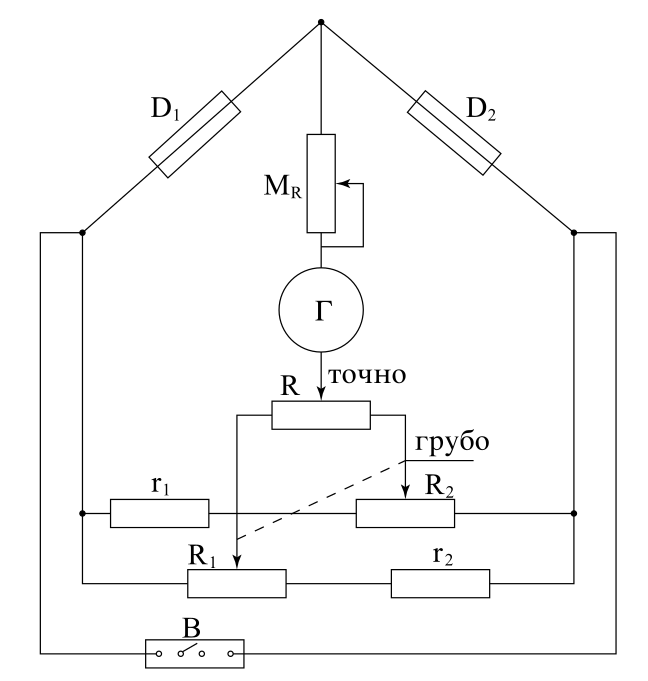
\includegraphics[width=7.5 cm]{scheme.png}
    \caption{Мостовая схема с датчиками теплопроводности для измерения разности концентраций газов}
    \label{picture:scheme}
\end{figure} 

Гелий содержится в баллоне (не изображен на рис. \ref{picture:ustan}) под давлением, превышающим атмосферное. Для предотвращения избыточного расхода гелия и его неконтролируемого проникания в установку предусмотрен металлический кран (К7), отделяющий её от баллона с гелием. Его открывают только на время непосредственного заполнения установки гелием, остальное время он должен быть закрыт. Для подачи малых порций гелия предусмотрен двухходовый кран с дозатором (рис. \ref{picture:crane}). При повороте рычажка Р в положение I гелий в небольшом количестве поступает в дозатор (если открыт К7), а при повороте Р в положение II порция из дозатора поступает в установку.

\begin{figure}[!h]
    \centering
    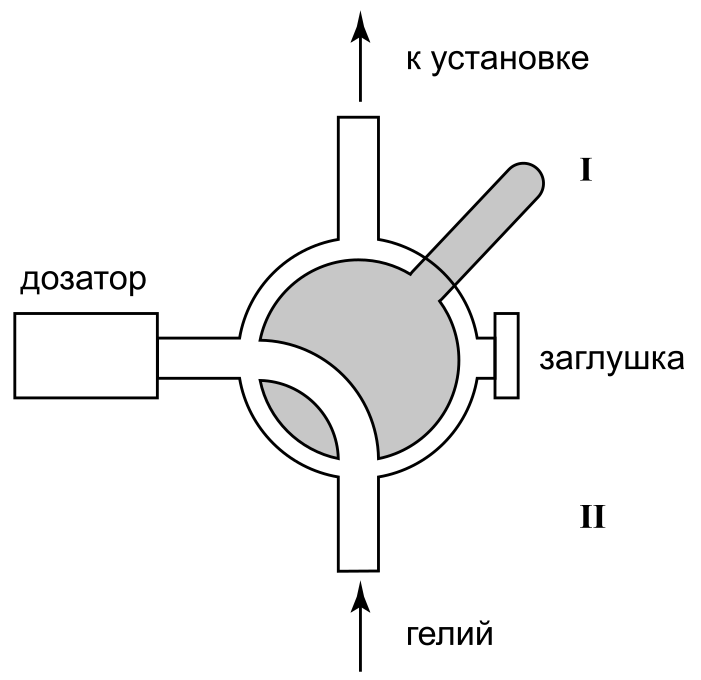
\includegraphics[width=7.5 cm]{crane.png}
    \caption{Кран $K_6$}
    \label{picture:crane}
\end{figure}

% \subsection*{Особенности установки}

% Кран $\text{К}_4$ изолирует форвакуумный насос от установки. Для подачи воздуха в установку служит кран $\text{К}_5$. Устройство и назначение кранов $\text{К}_6$ и $\text{К}_7$ подачи гелия соответствуют основному описанию. Дополнительный кран $\text{К'}_6$ служит для вакуумной изоляции установки от системы подачи гелия. Краны $\text{К}_4$, $\text{К}_5$ и $\text{К'}_6$ обладают повышенной вакуумплотностью и хорошо изолируют установку от протечек.

\section{Результаты измерений и обработка данных}

\subsection{Знакомство с установкой}

Познакомимся с установкой: изучим положение каждого крана на установке и всё остальное оборудование. Используется установка типа В (рис. \ref{picture:ustan}). Проверим, что компьютер включен и работает исправно.

Для данной установки известны следующие параметры:

\begin{equation}
    V_1 = (775 \pm 10) \ \text{см}^3, \ \ \ V_2 = (775 \pm 10) \ \text{см}^3, \ \ \ l/S = (5,3 \pm 0,1) \ 1/\text{см}
\end{equation}

\subsection{Подготовка оборудования}
\label{p:2}

Включим питание для всех приборов. Откроем краны К1, К2, К3. Убедимся, что кран К7 плотно закрыт.

Подсоединим установку в форвакуомному насосу. Откачаем её до давления $\sim$ 0,1 торр, для этого насос должен рботать в течение 3 минут. После откачки выключим насос.

\subsection{Балансировка измерительного моста}

Запустим в установку рабочее давление (в данном случае $P_\Sigma = 40$ торр). Изолируем объёмы $V_1$ и $V_2$ (закроем краны К1 и К2). Теперь сбалансируем измерительный мост с помощью переключателей грубо/точно так, чтобы напряжение на гальванометре было по модулю менее 0,1 мВ.

\subsection{Подготовка рабочих смесей}

Приготовим рабочие смеси для измерений. Для этого

\begin{enumerate}
    \item откачаем установку до $\sim$0,1 торр
    \item Изолируем объём $V_2$, закрыв краны К1 и К2
    \item Напусти в установку $P_{He} = 0,2 P_\text{раб}$ (в данном случае $\sim$8 торр или 1 деление на вакуометре)
    \item Перекроем подачу гелия и откачаем газ из патрубков (не забыв перекрыть кран К1)
    \item Откроем кран К2 и запустим в установку воздуха на $P_\text{В} = 1,675 P_\text{раб}$ (в данном случае 67 торр или 9 делений вакуометра)
    \item Уравняем давление в сосудах $V_1$ и $V_2$, открыв краны К1 и К2 и подождав 30 секунд.
    \item Запишем получившееся значение рабочего давления $P_\Sigma = 41_3$ торр
\end{enumerate}

\subsection{Измерения при процессе диффузии}
\label{p:5}

Запутим программу для сбора данных на компьютере, вобъём туда рабочее значение давления. Теперь откроем кран К3, подождём 2-3 секунды и запустим процесс измерения. Измеряем до тех пор, пока значение на гальванометре не упадёт на 50 \%. После измерения сохраним данные в папку (данные в здесь не представлены ввиду большого количества точек).

\subsection{Прочие измерения}

Проведём измерения, аналогичные пунктам \ref{p:2}-\ref{p:5}, только для рабочих давлений в 80, 120 и 160 торр.

\subsection{Проверка независимости коэффициента диффузии от пропорций компонентов}
\label{p:7}

Данный пункт работы не выполнялся.

\subsection{Проверка выполнения законы \eqref{eq:7}}

Для проверки выполнения закона \eqref{eq:7} построи для каждого набора измерений график зависимости $\ln{U}$ от времени $T$. Если закон выполняется, то эта зависимость должна быть линейной. Значит можно воспользоваться МНК для нахождения наилучшей прямой для каждого набора точек. В данном случае $x = T$, а $y = \ln{U}$. Для аппроксимации наилучшей прямой воспользуемся формулой:

\begin{equation}\label{eq:mnk}
    k = \frac{\langle xy\rangle - \langle x \rangle \langle y \rangle}{\langle x^2 \rangle - \langle x \rangle^2},
    \ \text{а} \ \  b = \langle y \rangle - k\langle x \rangle
\end{equation}

Погрешности для $k$ и $b$ рассчитываются по формулам:

\begin{equation}
    \sigma_k = \frac{1}{\sqrt{n}} \sqrt{\frac{\langle y^2 \rangle - \langle y \rangle^2}{\langle x^2 \rangle - \langle x \rangle^2} - k^2}
\end{equation}

\begin{equation}
    \sigma_b = \sigma_k\sqrt{\langle x^2 \rangle - \langle x \rangle^2}
\end{equation}

Посчитаем для каждого набора измерений промежуточные значения МНК и запишем их в таблицу \ref{table:mnk}.

\newpage

\begin{table}[!h]
    \centering
    \begin{tabular}{|l|r|r|r|r|}
    \hline
        $P_\Sigma$, торр & 41,3 & 82,5 & 120 & 161,3 \\ \hline
        $T$, с & 62,525 & 137,173 & 190,499 & 278,500 \\ \hline
        $\ln(U)$ & 2,224 & 2,147 & 2,201 & 2,242 \\ \hline
        $T \cdot T$, $\text{с}^2$ & 5232 & 25119 & 48450 & 103509 \\ \hline
        $\ln(U) \cdot \ln(U)$ & 4,983 & 4,649 & 4,880 & 5,070 \\ \hline
        $T \cdot \ln(U)$, с & 132,158 & 278,871 & 397,878 & 591,465 \\ \hline
        $n$ & 126 & 275 & 382 & 558 \\ \hline
        $k$, $\text{с}^{-1}$ & -0,005219 & -0,002482 & -0,001755 & -0,001273 \\ \hline
        $\sigma_k$, $\text{с}^{-1}$ & 0,000001 & 0,000002 & 0,000002 & 0,000001 \\ \hline
        $b$ & 2,55038 & 2,4875 & 2,5350 & 2,5971 \\ \hline
        $\sigma_b$ & 0,00005 & 0,0002 & 0,0002 & 0,0001 \\ \hline
    \end{tabular}\caption{\textit{Вычисление промежуточных значений для МНК для всех серий опытов}}\label{table:mnk-1}
\end{table}

Для каждого набора измерений вычислим параметры прямой и запишем в таблицу \ref{table:mnk-1}.

\begin{equation*}
    k_{41,3} = \frac{132,158 - 62,525 \cdot 2,224}{5232 - {62,525}^2} \approx -0,005219 \ \ \text{с}^{-1}
\end{equation*}

\begin{equation*}
    \sigma_{k_{41,3}} = \frac{1}{\sqrt{126}} \sqrt{\frac{4,983 - {2,224}^2}{5232 - {62,525}^2} - ({-0,005219})^2} \approx 0,000001 \ \ \text{с}^{-1}
\end{equation*}

\begin{equation*}
    b_{41,3} = 2,224 - (-0,005219) \cdot 62,525 \approx 2,55038
\end{equation*}

\begin{equation*}
    \sigma_{b_{41,3}} = 0,000001 \cdot \sqrt{5232 - {62,525}^2} \approx 0,00005
\end{equation*}

\begin{equation*}
    k_{82,5} = \frac{278,871 - 137,173 \cdot 2,147}{25119 - {137,173}^2} \approx -0,002482 \ \ \text{с}^{-1}
\end{equation*}

\begin{equation*}
    \sigma_{k_{82,5}} = \frac{1}{\sqrt{275}} \sqrt{\frac{4,649 - {2,147}^2}{25119 - {137,173}^2} - (-0,002482)^2} \approx 0,000002 \ \ \text{с}^{-1}
\end{equation*}

\begin{equation*}
    b_{82,5} = 2,147 - (-0,002482) \cdot 137,173 \approx 2,4875
\end{equation*}

\begin{equation*}
    \sigma_{b_{82,5}} = 0,000002 \cdot \sqrt{25119 - {137,173}^2} \approx 0,0002
\end{equation*}

\begin{equation*}
    k_{120} = \frac{397,878 - 190,499 \cdot 2,201}{48450 - {190,499}^2} \approx -0,001755 \ \ \text{с}^{-1}
\end{equation*}

\begin{equation*}
    \sigma_{k_{120}} = \frac{1}{\sqrt{382}} \sqrt{\frac{4,880 - {2,201}^2}{48450 - {190,499}^2} - (-0,001755)^2} \approx 0,000002 \ \ \text{с}^{-1}
\end{equation*}

\begin{equation*}
    b_{120} = 2,201 - (-0,001755) \cdot 190,499 \approx 2,5350
\end{equation*}

\begin{equation*}
    \sigma_{b_{120}} = 0,000002 \cdot \sqrt{48450 - {190,499}^2} \approx 0,0002
\end{equation*}

\begin{equation*}
    k_{161,3} = \frac{591,465 - 278,500 \cdot 2,242}{103509 - {278,500}^2} \approx -0,001273 \ \ \text{с}^{-1}
\end{equation*}

\begin{equation*}
    \sigma_{k_{161,3}} = \frac{1}{\sqrt{559}} \sqrt{\frac{5,070 - {2,242}^2}{103509 - {278,500}^2} - (-0,001273)^2} \approx 0,000001 \ \ \text{с}^{-1}
\end{equation*}

\begin{equation*}
    b_{161,3} = 2,242 - (-0,001273) \cdot 278,500 \approx 2,5971
\end{equation*}

\begin{equation*}
    \sigma_{b_{161,3}} = 0,000001 \cdot \sqrt{103509 - {278,500}^2} \approx 0,0001
\end{equation*}

Нанесём прямые на график, изображённый на рис. \ref{graph:1}. Экспериментальные точки наносить не будем, ввиду их количества.

\begin{figure}[h!]
        \centering
	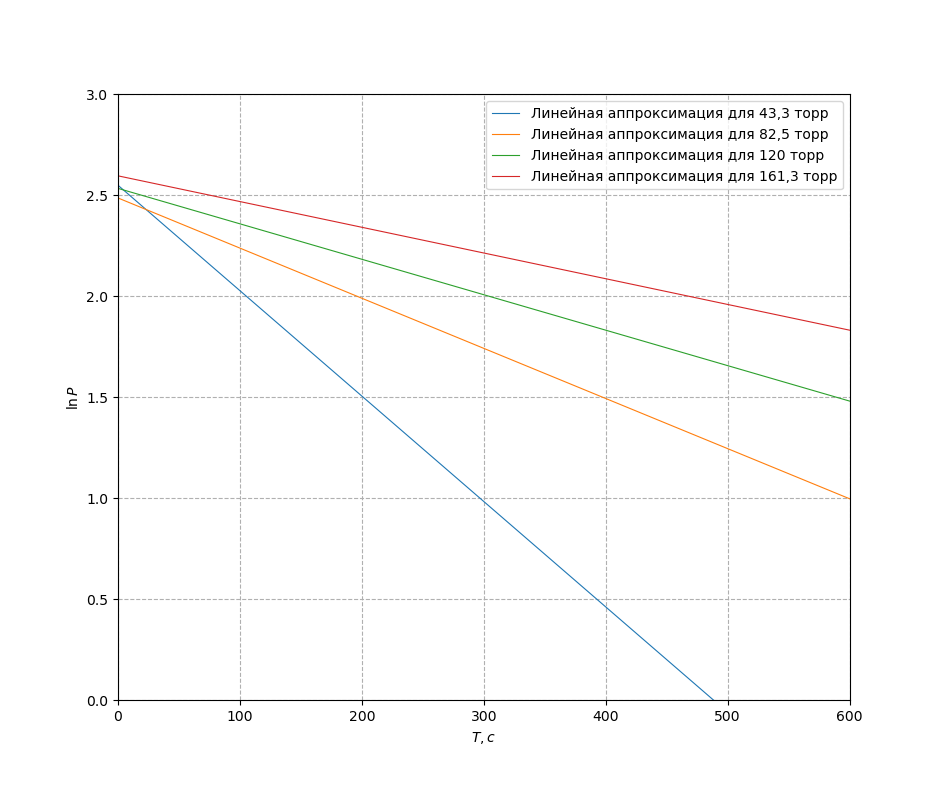
\includegraphics[width=1\textwidth]{graph_1.png}
	\caption{\textit{График зависимости $\ln{U}$ от $T$ для всех наборов измерений}}
	\label{graph:1}
\end{figure}

\newpage
Рассчитаем коэффициенты диффузии при выбранных рабочих давлениях. Так как мы имеем соотношение $\ln(U) = k t + b$, из которого получаем:

\begin{equation}
    U = U_0 e^{-t/\tau} \ \ \ \text{и} \ \ \ U = e^{kt + b} \implies U_0 = e^b, \ \ \ \ - \frac{1}{\tau} = k \implies \tau = - \frac{1}{k}
\end{equation}

Из формулы \eqref{eq:8} имеем:

\begin{equation}\label{eq:diffusion}
    D = \frac{V_1 V_2}{V_1 + V_2} \frac {l}{S \tau} = - \frac{V_1 V_2}{V_1 + V_2} \frac {kl}{S}
\end{equation}

Погрешность измерения $D$ можно вычислить по формуле:

\begin{equation*}
    \sigma_D = D \sqrt{
    \left( \frac{\partial D}{\partial V_1} \right)^2 (\sigma_{V_1})^2 + 
    \left( \frac{\partial D}{\partial V_2} \right)^2 (\sigma_{V_2})^2 + 
    \left( \frac{\partial D}{\partial l/S} \right)^2 (\sigma_{l/S})^2 + 
    \left( \frac{\partial D}{\partial k} \right)^2 (\sigma_{k})^2
    } = 
\end{equation*}
\begin{equation*}
    = D \sqrt{
    k^2 (l/S)^2 \frac{V_1^4\sigma_{V_2}^2 + V_2^4\sigma_{V_1}^2}{\left( V_1 + V_2 \right)^4} + 
    \frac{D^2}{(l/S)^2} \sigma_{l/S}^2 + \frac{D^2}{k^2} \sigma_{k}^2
    } = 
\end{equation*}
\begin{equation}\label{eq:diffusion_sigma}
    = D^2 \sqrt{
    \frac{\sigma_{V_1}^2 + \sigma_{V_2}^2}{\left( V_1 + V_2 \right)^2} + 
    \frac{\sigma_{l/S}^2}{(l/S)^2} + \frac{\sigma_{k}^2}{k^2}
    }
\end{equation}

Теперь по формулам \eqref{eq:diffusion} и \eqref{eq:diffusion_sigma} рассчитаем коэффициент диффузии и его погрешность для каждого рабочего давления и запишем в таблицу \ref{table:diffusion}.

\begin{equation*}
    D_{41,3} = \frac{775 \cdot 775}{775 + 775} \cdot 0,005219 \cdot 5,3 \approx 10,7 \ \text{см}^2 \cdot \text{с}^{-1}
\end{equation*}
\begin{equation*}
    \sigma_{D_{41,3}} = 11^2 \sqrt{
    \frac{10^2 + 10^2}{\left( 775 + 775 \right)^2} + 
    \frac{{0,1}^2}{{5,3}^2} + \frac{{0,000001}^2}{({-0,005219})^2}
    } \approx 0,2 \ \text{см}^2 \cdot \text{с}^{-1}
\end{equation*}

\begin{equation*}
    D_{82,5} = \frac{775 \cdot 775}{775 + 775} \cdot 0,002482 \cdot 5,3 \approx 5,1 \ \text{см}^2 \cdot \text{с}^{-1}
\end{equation*}
\begin{equation*}
    \sigma_{D_{82,5}} = {5,1}^2 \sqrt{
    \frac{10^2 + 10^2}{\left( 775 + 775 \right)^2} + 
    \frac{{0,1}^2}{{5,3}^2} + \frac{{0,000002}^2}{({-0,002482})^2}
    } \approx 0,1 \ \text{см}^2 \cdot \text{с}^{-1}
\end{equation*}

\begin{equation*}
    D_{120} = \frac{775 \cdot 775}{775 + 775} \cdot 0,001755 \cdot 5,3 \approx 3,6 \ \text{см}^2 \cdot \text{с}^{-1}
\end{equation*}
\begin{equation*}
    \sigma_{D_{120}} = {5,1}^2 \sqrt{
    \frac{10^2 + 10^2}{\left( 775 + 775 \right)^2} + 
    \frac{{0,1}^2}{{5,3}^2} + \frac{{0,000002}^2}{({-0,001755})^2}
    } \approx 0,1 \ \text{см}^2 \cdot \text{с}^{-1}
\end{equation*}

\begin{equation*}
    D_{161,3} = \frac{775 \cdot 775}{775 + 775} \cdot 0,001273 \cdot 5,3 \approx 2,6 \ \text{см}^2 \cdot \text{с}^{-1}
\end{equation*}
\begin{equation*}
    \sigma_{D_{161,3}} = {5,1}^2 \sqrt{
    \frac{10^2 + 10^2}{\left( 775 + 775 \right)^2} + 
    \frac{{0,1}^2}{{5,3}^2} + \frac{{0,000001}^2}{({-0,001273})^2}
    } \approx 0,1 \ \text{см}^2 \cdot \text{с}^{-1}
\end{equation*}

\begin{table}[!ht]
    \centering
    \begin{tabular}{|l|l|l|l|l|}
    \hline
        $P_\text{раб}$, торр & 41,3 & 82,5 & 120 & 161,3 \\ \hline
        $D$, $\text{см}^2 \text{с}^{-1}$ & 10,7 & 5,1 & 3,6 & 2,6 \\ \hline
        $\sigma_D$, $\text{см}^2 \text{с}^{-1}$ & 0,2 & 0,1 & 0,1 & 0,1 \\ \hline
    \end{tabular}\caption{\textit{Коэффициенты диффузии для соотвтетствующих значений давления}}\label{table:diffusion}
\end{table}

\newpage
 
\subsection{График зависимости коэффициента диффуизии от обратного давления}

Построим график зависимости коэффициента диффузии $D$ от обратного давления $1/P$. Так как зависимость должна быть линейной, то воспользуемся МНК, где $x = 1/P$, а $y = D$. Для параметров наилучшей прямой имеем:

\begin{equation}\label{eq:mnk-linear}
    k = \frac{\langle x y \rangle}{\langle x^2 \rangle}, \ \ \ \sigma_k = \frac{1}{\sqrt{n}} \sqrt{\frac{\langle y^2 \rangle}{\langle x^2 \rangle} - k^2}
\end{equation}

Посчитаем все промежуточные значения МНК и запишем их в таблицу \ref{table:mnk-2}.

\begin{table}[!ht]
    \centering
    \begin{tabular}{|l|l|l|l|l|l|}
    \hline
        $N$ & $x$ & $y$ & $x^2$ & $y^2$ & $xy$ \\ \hline
        1 & 0,024 & 11 & 0,00059 & 114,9 & 0,26 \\ \hline
        2 & 0,012 & 5,1 & 0,00015 & 26,0 & 0,06 \\ \hline
        3 & 0,008 & 3,6 & 0,00007 & 13,0 & 0,03 \\ \hline
        4 & 0,006 & 2,6 & 0,00004 & 6,8 & 0,02 \\ \hline
        ср & 0,013 & 5,5 & 0,00021 & 40,2 & 0,09 \\ \hline
    \end{tabular}\caption{\textit{Вычисление промежуточных значений МНК для зависимости $D$ от $1/P$}}\label{table:mnk-2}
\end{table}

Теперь посчитаем по формуле \eqref{eq:mnk-linear} параметры прямой:

\begin{equation*}
    k_D = \frac{0,09}{0,00021} \approx 437 \ \text{торр} \cdot \text{см}^2 \cdot \text{с}^{-1}
\end{equation*}
\begin{equation*}
    \sigma_{k_D} = \frac{1}{\sqrt{4}} \sqrt{\frac{40,2}{0,00021} - 437^2} \approx 5 \ \text{торр} \cdot \text{см}^2 \cdot \text{с}^{-1}
\end{equation*}

Нанесём график этой прямой на рис. \ref{graph:2}.

Теперь пользуясь полученной зависимостью вычислим значение коэффициента диффузии при атмосферном давлении $P_A = 753,5$ торр:

\begin{equation*}
    D_A = k_D / P_A = 437 / 753,5 \approx 0,580 \ \text{торр} \cdot \text{см}^2 \cdot \text{с}^{-1}
\end{equation*}
\begin{equation*}
    \sigma_{D_A} = D_A \sqrt{
    \frac{\sigma_{k_D}^2}{k_D^2} + \frac{\sigma_{P_A}^2}{P_A^2}} = 0,580 \sqrt{
    \frac{5^2}{437^2} + \frac{{0,3}^2}{{753,5}^2}
    } \approx 0,006 \ \text{торр} \cdot \text{см}^2 \cdot \text{с}^{-1}
\end{equation*}

Тогда

\begin{equation}
    D_A = (580 \pm 6) \cdot 10^{-3} \ \text{торр} \cdot \text{см}^2 \cdot \text{с}^{-1}
\end{equation}

Табличное значение $D_A^\text{табл} = 620 \cdot 10^{-3} \ \text{торр} \cdot \text{см}^2 \cdot \text{с}^{-1}$. Как видно полученное экспериментально значение неплохо совпадает с табличным.

\begin{figure}[h!]
        \centering
	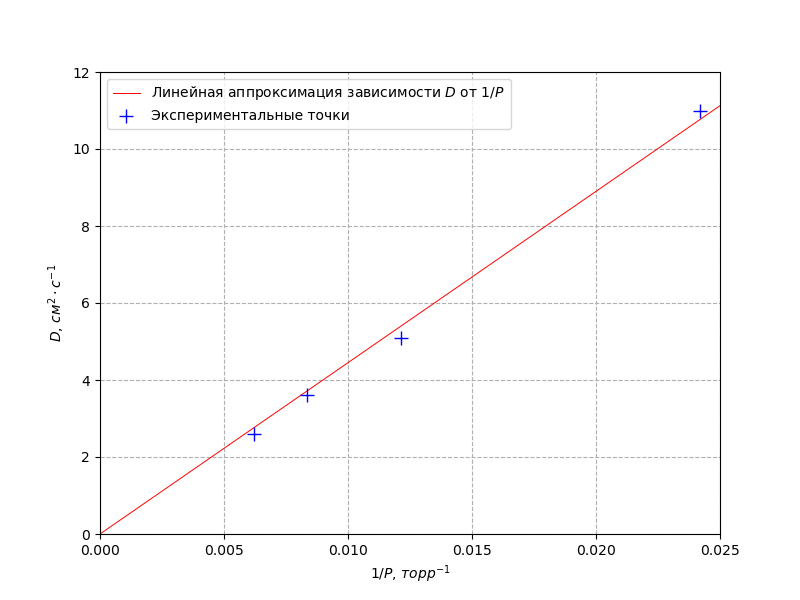
\includegraphics[width=1\textwidth]{graph_2.png}
	\caption{\textit{График зависимости $D$ от $1/P$}}
	\label{graph:2}
\end{figure}

\newpage

\subsection{Сравнение коэффециентов диффузии}

Данный пункт работы не выполняется, так как не выполнялся пункт \ref{p:7}.

\subsection{Оценка длины свободного пробега атомов гелия  и эффективного сечения столкновения атомов гелия с молекулами воздуха}


Оценим эффективное сечение столкновения атомов гелия с молекулами воздуха:

\begin{equation}
    \sigma = \pi \left( R_{He} + R_{N2} \right)^2 = 3,14 \cdot \left( 1,67824 \cdot 10^{-15} + 0,38 \cdot 10^{-9} \right)^2 \approx 4,5 \cdot 10^{-19} \ \text{м}^2
\end{equation}

Вычислим среднюю тепловую скорость молекул гелия:

\begin{equation*}
    \overline{v} = \sqrt{\frac{8RT}{\pi \mu}} = \sqrt{\frac{8 \cdot 8,31 \cdot 296}{3,14 \cdot 4 \cdot 10^{-3}}} \approx 1250 \ \frac{\text{м}}{\text{с}}
\end{equation*}

Из формулы \eqref{eq:2} получаем:

\begin{equation*}
    \lambda_{He} = \frac{3D_A}{\overline{v}} = \frac{3 \cdot 0,58 \cdot 133 \cdot 10^{-4}}{1250} \approx 1,9 \cdot 10^{-5} \ \text{м}
\end{equation*}

\section{Обсуждение результатов и выводы}

В ходе работы была зарегистрирована зависимость концентрации гелия в воздухе от времени с помощью датчиков теплопроводности для четырёх рабочих значений давления.

Были измерены коэффициенты диффузии при рабочих давлениях. Было экстраполировано значение коэффициента диффузии при нормальных условиях, которое приблизительно совпадает с табличным значением.

Были оценены величины длины свободного пробега атомов гелия  и эффективного сечения столкновения атомов гелия с молекулами воздуха.

\end{document}